% Created by tikzDevice version 0.11 on 2018-04-15 12:26:52
% !TEX encoding = UTF-8 Unicode
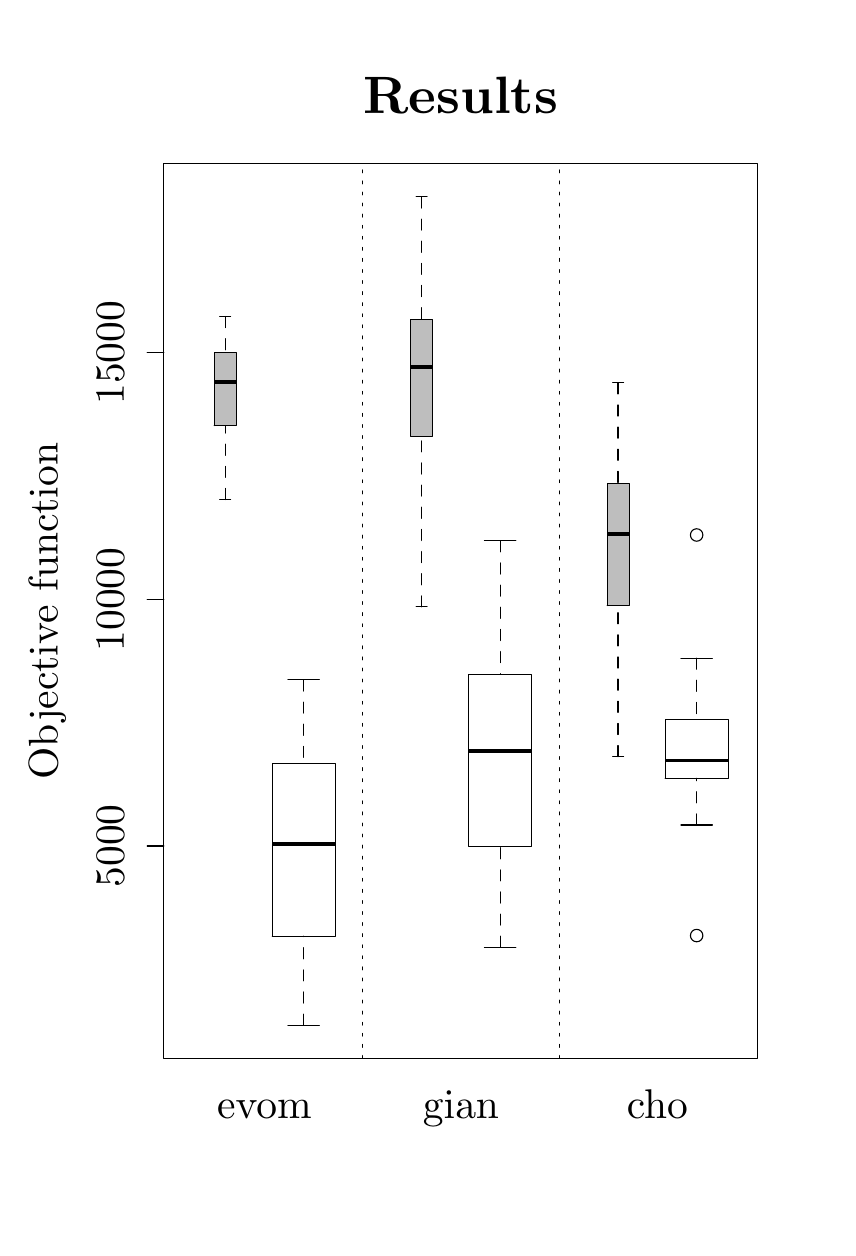
\begin{tikzpicture}[x=1pt,y=1pt]
\definecolor{fillColor}{RGB}{255,255,255}
\path[use as bounding box,fill=fillColor,fill opacity=0.00] (0,0) rectangle (289.08,433.62);
\begin{scope}
\path[clip] ( 49.20, 61.20) rectangle (263.88,384.42);
\definecolor{fillColor}{RGB}{190,190,190}

\path[fill=fillColor] ( 67.37,289.82) --
	( 75.33,289.82) --
	( 75.33,316.10) --
	( 67.37,316.10) --
	cycle;
\definecolor{drawColor}{RGB}{0,0,0}

\path[draw=drawColor,line width= 1.2pt,line join=round] ( 67.37,305.56) -- ( 75.33,305.56);

\path[draw=drawColor,line width= 0.4pt,dash pattern=on 4pt off 4pt ,line join=round,line cap=round] ( 71.35,263.11) -- ( 71.35,289.82);

\path[draw=drawColor,line width= 0.4pt,dash pattern=on 4pt off 4pt ,line join=round,line cap=round] ( 71.35,329.23) -- ( 71.35,316.10);

\path[draw=drawColor,line width= 0.4pt,line join=round,line cap=round] ( 69.36,263.11) -- ( 73.34,263.11);

\path[draw=drawColor,line width= 0.4pt,line join=round,line cap=round] ( 69.36,329.23) -- ( 73.34,329.23);

\path[draw=drawColor,line width= 0.4pt,line join=round,line cap=round] ( 67.37,289.82) --
	( 75.33,289.82) --
	( 75.33,316.10) --
	( 67.37,316.10) --
	( 67.37,289.82);
\definecolor{fillColor}{RGB}{255,255,255}

\path[fill=fillColor] ( 88.39,105.37) --
	(111.11,105.37) --
	(111.11,167.75) --
	( 88.39,167.75) --
	cycle;

\path[draw=drawColor,line width= 1.2pt,line join=round] ( 88.39,138.63) -- (111.11,138.63);

\path[draw=drawColor,line width= 0.4pt,dash pattern=on 4pt off 4pt ,line join=round,line cap=round] ( 99.75, 73.17) -- ( 99.75,105.37);

\path[draw=drawColor,line width= 0.4pt,dash pattern=on 4pt off 4pt ,line join=round,line cap=round] ( 99.75,197.92) -- ( 99.75,167.75);

\path[draw=drawColor,line width= 0.4pt,line join=round,line cap=round] ( 94.07, 73.17) -- (105.43, 73.17);

\path[draw=drawColor,line width= 0.4pt,line join=round,line cap=round] ( 94.07,197.92) -- (105.43,197.92);

\path[draw=drawColor,line width= 0.4pt,line join=round,line cap=round] ( 88.39,105.37) --
	(111.11,105.37) --
	(111.11,167.75) --
	( 88.39,167.75) --
	( 88.39,105.37);
\definecolor{fillColor}{RGB}{190,190,190}

\path[fill=fillColor] (138.37,286.01) --
	(146.32,286.01) --
	(146.32,328.30) --
	(138.37,328.30) --
	cycle;

\path[draw=drawColor,line width= 1.2pt,line join=round] (138.37,311.00) -- (146.32,311.00);

\path[draw=drawColor,line width= 0.4pt,dash pattern=on 4pt off 4pt ,line join=round,line cap=round] (142.34,224.32) -- (142.34,286.01);

\path[draw=drawColor,line width= 0.4pt,dash pattern=on 4pt off 4pt ,line join=round,line cap=round] (142.34,372.45) -- (142.34,328.30);

\path[draw=drawColor,line width= 0.4pt,line join=round,line cap=round] (140.35,224.32) -- (144.33,224.32);

\path[draw=drawColor,line width= 0.4pt,line join=round,line cap=round] (140.35,372.45) -- (144.33,372.45);

\path[draw=drawColor,line width= 0.4pt,line join=round,line cap=round] (138.37,286.01) --
	(146.32,286.01) --
	(146.32,328.30) --
	(138.37,328.30) --
	(138.37,286.01);
\definecolor{fillColor}{RGB}{255,255,255}

\path[fill=fillColor] (159.38,137.89) --
	(182.10,137.89) --
	(182.10,199.95) --
	(159.38,199.95) --
	cycle;

\path[draw=drawColor,line width= 1.2pt,line join=round] (159.38,172.19) -- (182.10,172.19);

\path[draw=drawColor,line width= 0.4pt,dash pattern=on 4pt off 4pt ,line join=round,line cap=round] (170.74,101.31) -- (170.74,137.89);

\path[draw=drawColor,line width= 0.4pt,dash pattern=on 4pt off 4pt ,line join=round,line cap=round] (170.74,248.18) -- (170.74,199.95);

\path[draw=drawColor,line width= 0.4pt,line join=round,line cap=round] (165.06,101.31) -- (176.42,101.31);

\path[draw=drawColor,line width= 0.4pt,line join=round,line cap=round] (165.06,248.18) -- (176.42,248.18);

\path[draw=drawColor,line width= 0.4pt,line join=round,line cap=round] (159.38,137.89) --
	(182.10,137.89) --
	(182.10,199.95) --
	(159.38,199.95) --
	(159.38,137.89);
\definecolor{fillColor}{RGB}{190,190,190}

\path[fill=fillColor] (209.36,224.79) --
	(217.31,224.79) --
	(217.31,268.80) --
	(209.36,268.80) --
	cycle;

\path[draw=drawColor,line width= 1.2pt,line join=round] (209.36,250.64) -- (217.31,250.64);

\path[draw=drawColor,line width= 0.4pt,dash pattern=on 4pt off 4pt ,line join=round,line cap=round] (213.33,170.21) -- (213.33,224.79);

\path[draw=drawColor,line width= 0.4pt,dash pattern=on 4pt off 4pt ,line join=round,line cap=round] (213.33,305.28) -- (213.33,268.80);

\path[draw=drawColor,line width= 0.4pt,line join=round,line cap=round] (211.35,170.21) -- (215.32,170.21);

\path[draw=drawColor,line width= 0.4pt,line join=round,line cap=round] (211.35,305.28) -- (215.32,305.28);

\path[draw=drawColor,line width= 0.4pt,line join=round,line cap=round] (209.36,224.79) --
	(217.31,224.79) --
	(217.31,268.80) --
	(209.36,268.80) --
	(209.36,224.79);
\definecolor{fillColor}{RGB}{255,255,255}

\path[fill=fillColor] (230.37,162.38) --
	(253.09,162.38) --
	(253.09,183.52) --
	(230.37,183.52) --
	cycle;

\path[draw=drawColor,line width= 1.2pt,line join=round] (230.37,168.93) -- (253.09,168.93);

\path[draw=drawColor,line width= 0.4pt,dash pattern=on 4pt off 4pt ,line join=round,line cap=round] (241.73,145.51) -- (241.73,162.38);

\path[draw=drawColor,line width= 0.4pt,dash pattern=on 4pt off 4pt ,line join=round,line cap=round] (241.73,205.80) -- (241.73,183.52);

\path[draw=drawColor,line width= 0.4pt,line join=round,line cap=round] (236.05,145.51) -- (247.41,145.51);

\path[draw=drawColor,line width= 0.4pt,line join=round,line cap=round] (236.05,205.80) -- (247.41,205.80);

\path[draw=drawColor,line width= 0.4pt,line join=round,line cap=round] (230.37,162.38) --
	(253.09,162.38) --
	(253.09,183.52) --
	(230.37,183.52) --
	(230.37,162.38);

\path[draw=drawColor,line width= 0.4pt,line join=round,line cap=round] (241.73,105.55) circle (  2.25);

\path[draw=drawColor,line width= 0.4pt,line join=round,line cap=round] (241.73,250.30) circle (  2.25);
\end{scope}
\begin{scope}
\path[clip] (  0.00,  0.00) rectangle (289.08,433.62);
\definecolor{drawColor}{RGB}{0,0,0}

\node[text=drawColor,rotate= 90.00,anchor=base,inner sep=0pt, outer sep=0pt, scale=  1.50] at ( 10.80,222.81) {Objective function};
\end{scope}
\begin{scope}
\path[clip] ( 49.20, 61.20) rectangle (263.88,384.42);
\definecolor{drawColor}{RGB}{0,0,0}

\path[draw=drawColor,line width= 0.4pt,dash pattern=on 1pt off 3pt ,line join=round,line cap=round] (121.04, 61.20) -- (121.04,384.42);

\path[draw=drawColor,line width= 0.4pt,dash pattern=on 1pt off 3pt ,line join=round,line cap=round] (192.04, 61.20) -- (192.04,384.42);
\end{scope}
\begin{scope}
\path[clip] (  0.00,  0.00) rectangle (289.08,433.62);
\definecolor{drawColor}{RGB}{0,0,0}

\node[text=drawColor,anchor=base,inner sep=0pt, outer sep=0pt, scale=  1.50] at ( 85.55, 39.60) {evom};

\node[text=drawColor,anchor=base,inner sep=0pt, outer sep=0pt, scale=  1.50] at (156.54, 39.60) {gian};

\node[text=drawColor,anchor=base,inner sep=0pt, outer sep=0pt, scale=  1.50] at (227.53, 39.60) {cho};
\end{scope}
\begin{scope}
\path[clip] (  0.00,  0.00) rectangle (289.08,433.62);
\definecolor{drawColor}{RGB}{0,0,0}

\node[text=drawColor,anchor=base,inner sep=0pt, outer sep=0pt, scale=  1.90] at (156.54,402.46) {\bfseries Results};
\end{scope}
\begin{scope}
\path[clip] (  0.00,  0.00) rectangle (289.08,433.62);
\definecolor{drawColor}{RGB}{0,0,0}

\path[draw=drawColor,line width= 0.4pt,line join=round,line cap=round] ( 49.20,137.92) -- ( 49.20,316.13);

\path[draw=drawColor,line width= 0.4pt,line join=round,line cap=round] ( 49.20,137.92) -- ( 43.20,137.92);

\path[draw=drawColor,line width= 0.4pt,line join=round,line cap=round] ( 49.20,227.02) -- ( 43.20,227.02);

\path[draw=drawColor,line width= 0.4pt,line join=round,line cap=round] ( 49.20,316.13) -- ( 43.20,316.13);

\node[text=drawColor,rotate= 90.00,anchor=base,inner sep=0pt, outer sep=0pt, scale=  1.50] at ( 34.80,137.92) {5000};

\node[text=drawColor,rotate= 90.00,anchor=base,inner sep=0pt, outer sep=0pt, scale=  1.50] at ( 34.80,227.02) {10000};

\node[text=drawColor,rotate= 90.00,anchor=base,inner sep=0pt, outer sep=0pt, scale=  1.50] at ( 34.80,316.13) {15000};

\path[draw=drawColor,line width= 0.4pt,line join=round,line cap=round] ( 49.20, 61.20) --
	(263.88, 61.20) --
	(263.88,384.42) --
	( 49.20,384.42) --
	( 49.20, 61.20);
\end{scope}
\end{tikzpicture}
